\chapter{Methodology}
\label{methodology}
In this chapter the basic principles for the following chapters will be explained.
The Section \ref{sec:docrep} describes how documents can be numerically represented. Section \ref{sec:topicmodel} then will introduce the topic modeling methods \ac{LDA} and \ac{NMF} which are used in this thesis.

\section{Document representation}
\label{sec:docrep}

\subsection{Bag of Words}
The Bag of Words \ac{BoW} model serves as a numerical representation of a document, which is used as input for further \ac{NLP} tasks.
It represents the document simply by the counts for each word. The grammar and the ordering of the words are ignored, so some information is lost. The document \textit{John likes organic but Mary doesn't} and the document {Mary likes organic but John doesn't} have the same \ac{BoW} representation although these differ in context. Nevertheless, similar \ac{BoW} imply similar document content (\cite{Manning2008}). 

\subsection{Tf-Idf Weighting}
Only considering the absolute term frequency ($tf_{t,d}$) of words is not the best measure to make differentiations between documents, because not all terms are equally important. 
The term \textit{organic} appears in  224 of 239 articles in the New York Times, obviously this term can not be considered as a stop word, however it is not suitable to differentiate the articles. Therefore the effect of the frequent words is reduced by the \textit{inverse document frequency}:
\begin{equation}
idf_{d,t} = log\dfrac{N_{d}}{df_{d,t}}
\end{equation}
%$$ idf_{d,t} = log\dfrac{N_{d}}{df_{d,t}} $$
$N_{d}$ is the number of all documents in a corpus, while $df_{d,t}$ is the number of documents that contain the single term.\\
Based on the term frequency $tf_{t,d}$ and the inverse document frequency $idf_{d,t}$ we introduce the \textit{\ac{tfidf}}: 

\begin{equation}
tf-idf_{d,t} = tf_{t,d} * idf_{t,d}
\end{equation}
%$$ tf-idf_{d,t} = tf_{t,d} * idf_{t,d}$$

The \ac{tfidf} weighting has the highest score when the term occurs frequently within a small amount of documents. The score is lower when the term occurs rarely or too often in many documents (\cite{Jurafsky2009}).

\subsection{Vector space model}
The representation of documents in the same vector space is known as the vector space model. This was originally introduced for \ac{IR} operations like scoring documents on a query, document classification or clustering \cite{Salton1975}.\\
The vector space model forms with the documents \textit{$D_{i}$} and all unique terms \textit{$T_{j}$} the document term matrix \textit{C}. Each row of \textit{C} corresponds every single document of the corpus and each column the single unique terms. In \textit{$C_{ij}$} the weightings either as term frequency or \ac{tfidf} for each term over all documents is stored. \\
In Table \ref{tab:doc_term_lda} the term frequency and in Table \ref{tab:doc_term_nmf}  \ac{tfidf} is calculated from three sample documents: \textit{Doc 1: Organic is healthier then conventional food}, \textit{Doc 2: I buy organic} and \textit{Doc 3: Organic is wasted money}.
In this thesis both topic modeling algorithms take the document term matrix as input, but with different weightings. For \ac{LDA} the term frequency and for \ac{NMF} the \ac{tfidf} weighting  is used.\\
\begin{table}[h]
	\begin{tabular}{lcccccccccc}
		\toprule
		& organic & is & healthier & then & conventional & food & i &buy& wasted  & money \\ \midrule
		Doc1 & 1 	& 1  &      1      &  1   & 1 			 & 1  	& 0 &0  &  0   	&  0  \\
		Doc2 & 1 	& 0  &      0      &  0   & 0 			 & 0  	& 1 &1  &  1   	&  0  \\
		Doc3 & 1 	& 1  &      0      &  0   & 0 			 & 0  	& 0 &0  &  1    &  1   \\ \bottomrule
	\end{tabular}
	\caption[Sample term frequency matrix]{Document term matrix with term-frequency weighting as used by \ac{LDA}.}
	\label{tab:doc_term_lda}
\end{table}	

\begin{table}[h]
	\begin{tabular}{lllllllllll}
		\toprule
		& organic & is & healthier & then & conventional & food & i &buy& wasted  & money \\ \midrule
		Doc1 & 0 	& 0.45  &   0.45      &  0.45   &  	0		 & 0.34  	& 0 &0.27  &  0.45   	&  0  \\
		Doc2 & 0.65 	& 0  &      0      &  0   & 0.65			 & 0  	& 0 &0.39  &  0   	&  0  \\
		Doc3 & 0 	& 0  &      0      &  0   & 0 			 & 0 .44 	& 0.58 &0.34  &  0    &  0.58   \\ \bottomrule
	\end{tabular}
	\caption[Sample \ac{tfidf} matrix]{Document term matrix with \ac{tfidf} weighting as used by \ac{NMF}.}
	\label{tab:doc_term_nmf}
\end{table}


\section{Topic Modeling}
\label{sec:topicmodel}
Every day large amounts of information are collected and become available. The vast quantities of data make it difficult to access those information we are looking for. Therefore, we need methods that help us to organize, summarize and understand large collections of data. Topic Modeling refers to a set of methods that help us to process large document collections efficiently. A topic model takes a set of documents as the input and outputs topics, a set of recurring themes that are discussed in the collection, and the degree to which each document expresses these topics \citep{Blei2003}. The topics are the hidden thematic structure of the document collection. They are found by recurring patterns of co-occurring words.

Topic Models are based on the assumption that a document is composed of multiple topics. Any document of the text collection is a combination of all topics with different weights. Therefore, all documents of one corpus are composed of the same topics by varying their weights. The documents are modeled as a probability distribution over the topics. 

Just as documents are distributions over all topics, topics are distributions over all words in a document collection. Every word of the collection is present in every topic, however, with varying probabilities. Sorting the terms of a topic by their probability reveals a semantically meaningful interpretation.

\subsection{Latent Dirichlet Allocation}
Currently, the most used method for topic modeling is \acl{LDA}, which was introduced by \cite{Blei2003}. \ac{LDA} is a generative model, that describes how the documents are generated from existing topics. By applying inference it is possible to reverse the process and use \ac{LDA} to derive the topics from the document collection. Further, \ac{LDA} is also a probabilistic model which means that the resulting topics can be seen as a probability distribution.

The research on topic models was started by \cite{Deerwester1990} with their introduction of \ac{LSA}. \ac{LSA} was used to solve the issues of polysemy and synonymy when performing queries for information retrieval. With probabilistic \ac{LSA} (pLSA) \cite{Hofmann1999} provided a probabilistic formulation of \ac{LSA}. \ac{LDA} is an extension of pLSA to be able to model unseen documents. In pLSA the topic proportions for every document need to be known, which makes it unable to model documents outside the training set. In \ac{LDA} the topic proportions for every document are derived from a Dirichlet distribution, thus enabling it to generalize to documents outside the training collection.

After the successful introduction to analyze large document collections, \ac{LDA} was also applied in other domains such as computer vision to classify \citep{Fei-Fei2005} and build hierarchies of images \citep{Li2010}. In fact, the method was independently discovered by \cite{Pritchard2000} in their field of evolutionary biology to study population genetics. For the interested reader, \cite{Jelodar2017} presents a literature study on extensions of \ac{LDA} and applications to various datasets.

As described above \ac{LDA} assumes a generative process how the documents of a corpus arose from existing topics. We first describe the generative process before explaining how it can be reversed to derive topics from existing documents.

\ac{LDA} draws the per-document topic distribution and the topics themselves from a  Dirichlet distribution. Therefore, before explaining \ac{LDA} the Dirichlet distribution is introduced. 

The Dirichlet distribution can be seen as a distribution over distributions. When sampling from a k-dimensional Dirichlet distribution one receives a discrete distribution over k elements. This is visualized in Figure \ref{fig:dirichlet1}. Each distribution represents a draw from a 3-dimensional Dirichlet distribution.

Further, the Dirichlet distribution can be parametrized by $\alpha$. The parameter describes how the probability mass of the Dirichlet distribution is distributed over the k-elements. When drawing from a Dirichlet with a high alpha parameter the probabilities for each element of the drawn discrete distribution are roughly the same. When drawing from a Dirichlet with a small alpha, the probability mass of the resulting discrete distribution is divided among a few highly probable elements. Visually, a high $\alpha$ value leads to a distribution as shown on the left of Figure \ref{fig:dirichlet1}. A low value would lead to distributions as shown on the right.

\begin{figure}
	\centering
	
		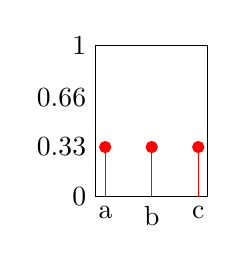
\begin{tikzpicture}
		\begin{axis}[
		width = 3cm,
		height = 3.5cm,
		symbolic x coords={a,b,c},
		xtick=data,
		ytick={0, 0.33, 0.66, 1},
		ymax=1,
		ymin=0,
		ytick style={draw=none},
		xtick style={draw=none}		
		]
		\addplot+[ycomb, color=red, mark options={red}] coordinates {(a,0.33) (b,0.33) (c,0.33)};
		\end{axis}
		\end{tikzpicture}
		\quad
		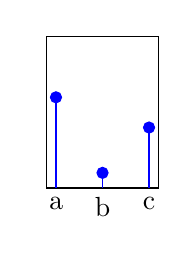
\begin{tikzpicture}
		\begin{axis}[
		width = 3cm,
		height = 3.5cm,
		symbolic x coords={a,b,c},
		xtick=data,
		yticklabels={,,},
		ymax=1,
		ymin=0,
		ytick style={draw=none},
		xtick style={draw=none}		
		]
		\addplot+[ycomb, color=blue, mark options={blue}] coordinates {(a,0.6) (b,0.1) (c,0.4)};
		\end{axis}
		\end{tikzpicture}
		\quad
		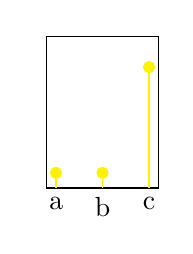
\begin{tikzpicture}
		\begin{axis}[
		width = 3cm,
		height = 3.5cm,
		symbolic x coords={a,b,c},
		xtick=data,
		ymax=1,
		ymin=0,
		ytick style={draw=none},
		xtick style={draw=none},
		yticklabels={,,}		
		]
		\addplot+[ycomb, color=yellow, mark options={yellow}] coordinates {(a,0.1) (b,0.1) (c,0.8)};
		\end{axis}
		\end{tikzpicture}
	\caption[Discrete distributions drawn from a 3-dimensional Dirichlet distribution]{Discrete distributions drawn from a 3-dimensional Dirichlet distribution. Adapted from \cite{Widmer2018}}
	\label{fig:dirichlet1}	
\end{figure}

Figure \ref{fig:dgmlda} represents \ac{LDA} as a graphical model. The grey nodes indicate observed variables, in this case the words $w$ of the documents. All white nodes are hidden variables that have to be derived. In topic modeling the hidden variables are the topic assignment $z_{w,d}$ of each word position $n$ in document $d$, the topic distribution $\theta_d$ for document $d$ and the word distribution $\phi_z$ for topic $z$. $\alpha$ and $\beta$ are hyper- parameters for the Dirichlet distribution on the per-document topic distribution and per-topic word distribution respectively.
With the introduced notation the generative process underlying \ac{LDA} can be described as follows:

\begin{itemize}
	\item From a Dirichlet distribution parametrized by $\alpha$ draw a multinomial distribution $\theta_d$ representing the topic proportions of document $d$. 
	\item For each word position $n$ in document $d$ choose a topic of the multinomial per-document topic distribution $\theta_d$. The chosen topic is the topic assignment $z_{n,d}$.
	\item From a Dirichlet distribution parametrized by $\beta$ draw a multinomial distribution $\phi_z$ representing the word proportions for topic $z$.
	\item The word $w$ at position $n$ in document $d$ is then drawn from the topic $z$. 
\end{itemize}

By applying this procedure for all documents and words we can generate the documents from existing topics. To derive the topics from existing documents we need to estimate the document-topic proportions $\theta$, the topics $\phi$ and the assignment of words to topics $z$ given the Dirichlet priors $\alpha$ and $\beta$ and the word of the documents $w$. This can be formulated as:
\begin{equation}
P(\theta, \phi, z| w, \alpha, \beta) = \frac{P(\theta, \phi, z, w |\alpha, \beta)}{P(w |\alpha, \beta)} 
\end{equation}

This fraction, however, is intractable to compute. Therefore, several approaches exist, such as Gibbs Sampling \citep{Griffiths2002}, Variational Inference \citep{Blei2003} or Expectation Propagation \citep{Minka2002}, to approximate the topic-term and document-topic distributions.

\begin{figure}
	\begin{tikzpicture}[x=1.7cm,y=1.8cm]
	
	% Nodes
	\node[obs] (W) {$w_{d,n}$} ; 
	\node[latent, left =of W] (Z) {$z_{d,n}$} ; 
	\node[latent, left =of Z] (TH) {$\theta_d$} ; 
	\node[const, left =of TH] (AL) {$\alpha$} ; 
	\node[latent, right =of W] (PH) {$\phi_k$} ; 
	\node[const, right =of PH] (BE) {$\beta$} ; 
	
	% Edges
	\edge {Z} {W} ; 
	\edge {TH} {Z}; 
	\edge {AL} {TH};
	\edge {PH} {W};
	\edge {BE} {PH};

	%Plates
	\plate {topicsPlate} {(PH)} {$K$} ; 
	\plate {wordsPlate} {(W) (Z)} {$N_d$} ; 
	\plate {documentsPlate} {(wordsPlate) (TH)} {$D$}
	
	%Description
	\node[ below= 2cm of AL, align=center] (A) {document\\hyperparameter} ;
	\node[ below= 3.5 cm of TH, align=center] (DTH) {per-document  \\topic distribution} ;
	\node[ below= 2cm of Z, align=center] (DZ) {per-word \\ topic assignment} ;
	\node[ below= 3.5cm of W, align=center] (DW) {observed \\ word} ;
	\node[ below= 2cm of PH, align=center] (DPH) {topics} ;
	\node[ below= 2cm of BE, align=center] (DBE) {topic \\ hyperparameter} ;
	\draw[dotted] (A) -- (AL) ;
	\draw[dotted] (DTH) -- (TH) ;
	\draw[dotted] (DZ) -- (Z) ;
	\draw[dotted] (DW) -- (W) ;
	\draw[dotted] (DPH) -- (PH) ;
	\draw[dotted] (DBE) -- (BE) ;
	\end{tikzpicture}
	

	\caption[Graphical model of \ac{LDA}]{Graphical model of \ac{LSA}. Adapted from \cite{Widmer2018}}
	\label{fig:dgmlda}
\end{figure}


\subsection{Non negative Matrix Factorization}

Apart from the probabilistic methods as described above, linear methods, such as \acl{NMF} have proven useful for topic modeling. \ac{NMF} was introduced by \cite{Lee1999} as a method for dimensionality reduction. They show that their method can lead to a lower dimensional parts-based representation with naturally interpretable components. When applied on a set of facial images, the parts resemble different portions of a human face. The original facial images can be reconstructed by combining the parts. This approach can also be applied on a set of textual documents. In this case the parts-based representation are the semantic topics of the documents and the documents can be reconstructed by combining the topics.

\ac{NMF} requires that the original data is non-negative. This is the case for the previously presented applications in computer vision and text mining. The pixel values of images or term counts of documents are always positive. It is also typical to data in other fields that they are non-negative. Therefore, \ac{NMF} was also successfully applied in spectral analysis \citep{Pauca2006} and bio-informatics\citep{Brunet2004}.

Formally, \ac{NMF} can be described as follows. Given a non-negative matrix $C \in \mathbb{R}_{\geq 0}^{n\times m}$ and a rank desired $k < min(m,n)$ find two non-negative matrices $W \in \mathbb{R}_{\geq 0}^{n \times k}$ and $H \in \mathbb{R}_{\geq 0}^{k \times m}$ so that the reconstruction error is minimized:
\begin{equation}
\min_{W,H} ||C - WH||_F
\end{equation}
In this case, the reconstruction error is measured by the Frobenius norm, which is an extension of the Euclidean form on matrices. The output and input of \ac{NMF} is similar to \ac{LDA}. Matrix $C$ is the original document term matrix whereas the matrices $W$ and $H$ represent the topic term respectively the document topic matrix. For every document $c$ there is a corresponding column $h$ in the document topic matrix $H$. The column contains the weights for each topic (columns of $W$) for this specific document. Thus, the document $c$ is modeled as a linear combination of the columns of $W$:
\begin{equation}
c \approx Wh
\end{equation}.
The similarity of \ac{LDA} and \ac{NMF} in terms of matrix factorization is evident from Figure \ref{fig:comparison}. However, there is an important difference in the interpretation of  the values in the generated matrices. With \ac{LDA} the outputted document-topic and topic-term matrices are probability distributions. \ac{NMF}, however, has no probabilistic interpretation and while returned values represent topic or term weights they do not necessarily sum up to 1. To circumvent this difference the output of \ac{NMF} was normalized. 

\begin{figure} 
	\centering
			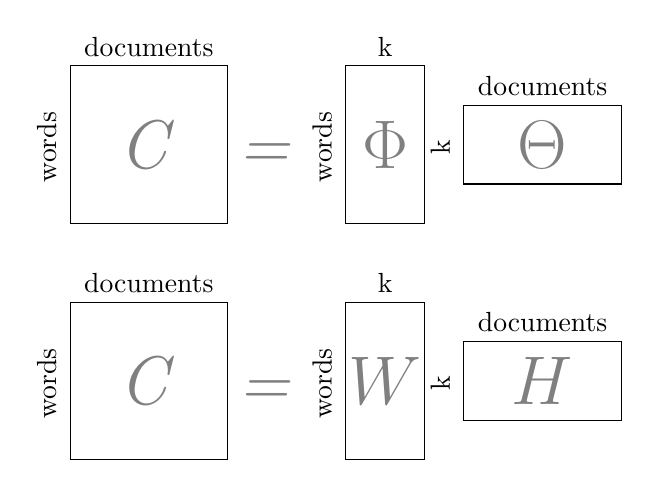
\begin{tikzpicture}
			
			% LDA
		 	\draw (0, 0) rectangle (2, 2);
		 	\node [above] at (1, 2) {documents};
		 	\node [right, rotate=90] at (-0.3, 0.4) {words};
		 	\node at (1, 1) {\Huge \color{gray} \textit{C}};
		 	\node at (2.5, 0.85) {\Huge \color{gray} \textit{=}};
		 	
		 	\draw (3.5, 0) rectangle (4.5, 2);
		 	\node [above] at (4, 2) {k};
		 	\node [right, rotate=90] at (3.2, 0.4) {words}; 
		 	\node at (4, 1) {\Huge \color{gray} $\Phi$};
		 	
		 	\draw (5, 0.5) rectangle (7, 1.5);
		 	\node [above] at (6, 1.5) {documents};
		 	\node [right, rotate=90] at (4.7, 0.75) {k}; 
		 	\node at (6, 1) {\Huge \color{gray} $\Theta$};
		 	
		 	% NMF
		 	\draw (0, -3) rectangle (2, -1);
		 	\node [above] at (1, -1) {documents};
		 	\node [right, rotate=90] at (-0.3, -2.6) {words};
		 	\node at (1, -2) {\Huge \color{gray} \textit{C}};
		 	\node at (2.5, -2.15) {\Huge \color{gray} \textit{=}};
		 	
		 	\draw (3.5, -3) rectangle (4.5, -1);
		 	\node [above] at (4, -1) {k};
		 	\node [right, rotate=90] at (3.2, -2.6) {words}; 
		 	\node at (4, -2) {\Huge \color{gray}  $W$};
		 	
		 	\draw (5, -2.5) rectangle (7, -1.5);
		 	\node [above] at (6, -1.5) {documents};
		 	\node [right, rotate=90] at (4.7, -2.25) {k}; 
		 	\node at (6, -2) {\Huge \color{gray} $H$};
	
\end{tikzpicture}
		 	

	\caption[Similarity of LSA and NMF from the perspective of matrix decomposition]{Showing the similarity of \ac{LDA}, and \ac{NMF} from the perspective of matrix decomposition. Adapted from \cite{Steyvers2007a}.}
	\label{fig:comparison} 
\end{figure} 
